\documentclass[tikz,border=9pt]{standalone}
\usepackage{amsmath,amssymb}
\usetikzlibrary{arrows.meta,positioning,calc}
\begin{document}
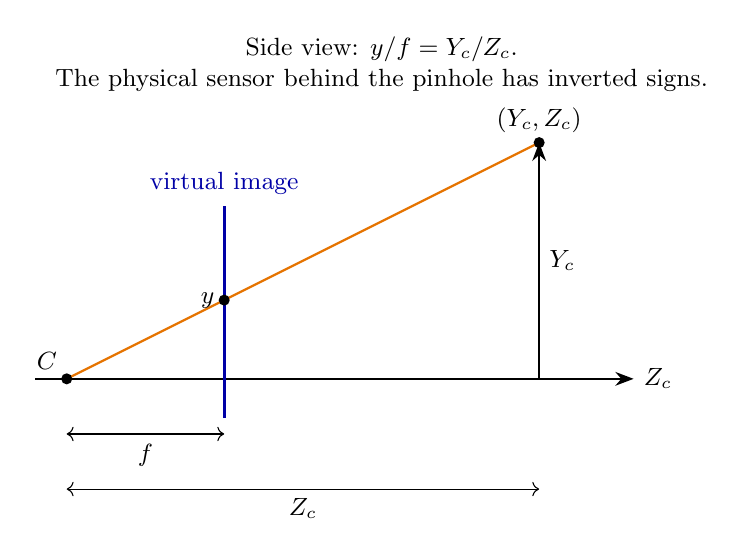
\begin{tikzpicture}[font=\small,arr/.style={-{Stealth},thick},box/.style={draw=blue!55!black,rounded corners,fill=blue!4,align=center,text width=2.9cm,minimum height=1.05cm}]

\coordinate (C) at (0,0);\coordinate (x) at (2,1);\coordinate (X) at (6,3);
\draw[arr] (-.4,0)--(7.2,0) node[right]{$Z_c$};
\draw[blue!65!black,very thick] (2,-.5)--(2,2.2) node[above]{virtual image};
\draw[arr,thick] (6,0)--(X) node[midway,right]{$Y_c$};
\draw[thick,orange!90!black] (C)--(X);
\draw[<->] (0,-.7)--(2,-.7) node[midway,below]{$f$};
\draw[<->] (0,-1.4)--(6,-1.4) node[midway,below]{$Z_c$};
\fill (C) circle(2pt) node[above left]{$C$};\fill (x) circle(2pt) node[left]{$y$};\fill (X) circle(2pt) node[above]{$(Y_c,Z_c)$};
\node[align=center] at (4,4){Side view: $y/f=Y_c/Z_c$.\\The physical sensor behind the pinhole has inverted signs.};

\end{tikzpicture}
\end{document}
